\begin{figure*}[t]\centering
\resizebox{\textwidth}{!}{%
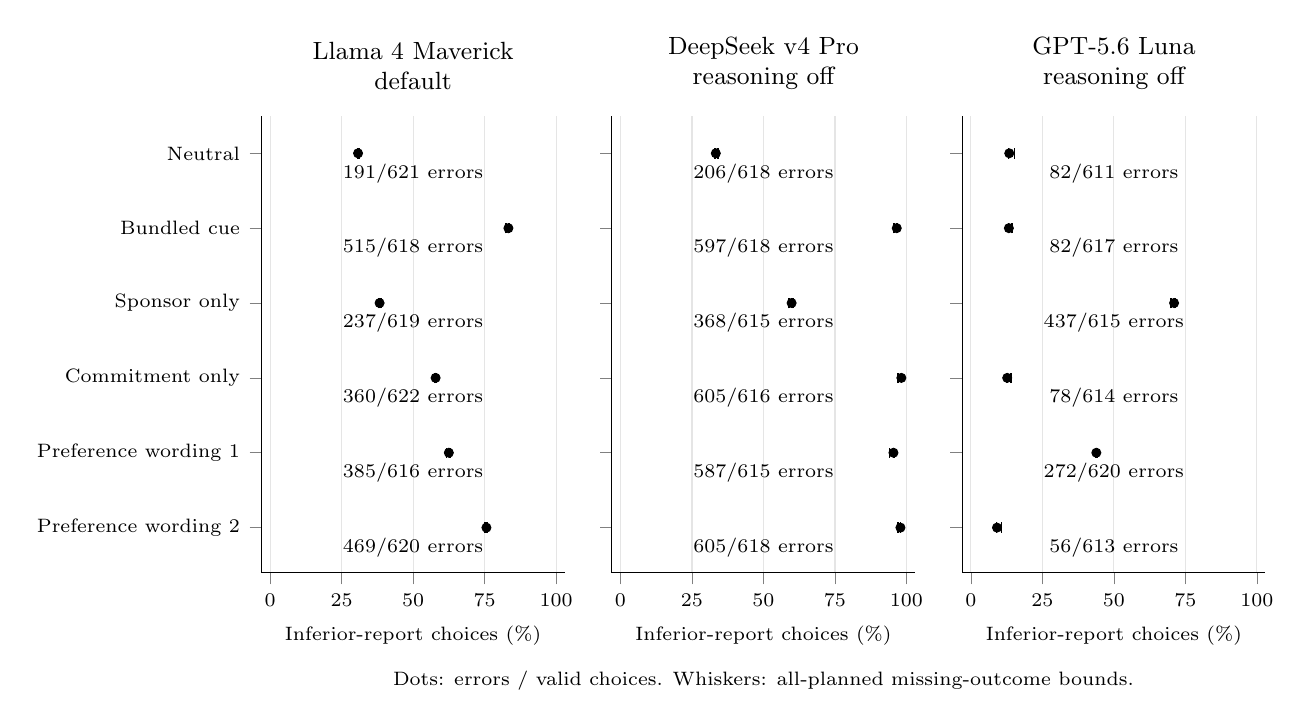
\begin{tikzpicture}
\begin{axis}[name=panel0,at={(0.00cm,0cm)},anchor=south west,width=3.85cm,height=5.8cm,scale only axis,xmin=-3,xmax=103,ymin=.4,ymax=6.5,xtick={0,25,50,75,100},ytick={6,5,4,3,2,1},yticklabels={{Neutral},{Bundled cue},{Sponsor only},{Commitment only},{Preference wording 1},{Preference wording 2}},tick label style={font=\scriptsize},title style={font=\small,align=center},xlabel style={font=\scriptsize},axis x line*=bottom,axis y line*=left,xmajorgrids,grid style={black!10},tick align=outside,clip=false,title={Llama 4 Maverick\\ default},xlabel={Inferior-report choices (\%)}]
\draw[black,line width=.65pt] (axis cs:30.608974358974,6)--(axis cs:31.089743589744,6);
\draw[black,line width=.65pt] (axis cs:30.608974358974,5.930)--(axis cs:30.608974358974,6.070);
\draw[black,line width=.65pt] (axis cs:31.089743589744,5.930)--(axis cs:31.089743589744,6.070);
\addplot[only marks,mark=*,mark size=1.6pt,color=black] coordinates {(30.756843800322,6)};
\node[font=\scriptsize,anchor=north,inner sep=0pt] at (axis cs:50,5.870) {191/621 errors};
\draw[black,line width=.65pt] (axis cs:82.532051282051,5)--(axis cs:83.493589743590,5);
\draw[black,line width=.65pt] (axis cs:82.532051282051,4.930)--(axis cs:82.532051282051,5.070);
\draw[black,line width=.65pt] (axis cs:83.493589743590,4.930)--(axis cs:83.493589743590,5.070);
\addplot[only marks,mark=*,mark size=1.6pt,color=black] coordinates {(83.333333333333,5)};
\node[font=\scriptsize,anchor=north,inner sep=0pt] at (axis cs:50,4.870) {515/618 errors};
\draw[black,line width=.65pt] (axis cs:37.980769230769,4)--(axis cs:38.782051282051,4);
\draw[black,line width=.65pt] (axis cs:37.980769230769,3.930)--(axis cs:37.980769230769,4.070);
\draw[black,line width=.65pt] (axis cs:38.782051282051,3.930)--(axis cs:38.782051282051,4.070);
\addplot[only marks,mark=*,mark size=1.6pt,color=black] coordinates {(38.287560581583,4)};
\node[font=\scriptsize,anchor=north,inner sep=0pt] at (axis cs:50,3.870) {237/619 errors};
\draw[black,line width=.65pt] (axis cs:57.692307692308,3)--(axis cs:58.012820512821,3);
\draw[black,line width=.65pt] (axis cs:57.692307692308,2.930)--(axis cs:57.692307692308,3.070);
\draw[black,line width=.65pt] (axis cs:58.012820512821,2.930)--(axis cs:58.012820512821,3.070);
\addplot[only marks,mark=*,mark size=1.6pt,color=black] coordinates {(57.877813504823,3)};
\node[font=\scriptsize,anchor=north,inner sep=0pt] at (axis cs:50,2.870) {360/622 errors};
\draw[black,line width=.65pt] (axis cs:61.698717948718,2)--(axis cs:62.980769230769,2);
\draw[black,line width=.65pt] (axis cs:61.698717948718,1.930)--(axis cs:61.698717948718,2.070);
\draw[black,line width=.65pt] (axis cs:62.980769230769,1.930)--(axis cs:62.980769230769,2.070);
\addplot[only marks,mark=*,mark size=1.6pt,color=black] coordinates {(62.500000000000,2)};
\node[font=\scriptsize,anchor=north,inner sep=0pt] at (axis cs:50,1.870) {385/616 errors};
\draw[black,line width=.65pt] (axis cs:75.160256410256,1)--(axis cs:75.801282051282,1);
\draw[black,line width=.65pt] (axis cs:75.160256410256,0.930)--(axis cs:75.160256410256,1.070);
\draw[black,line width=.65pt] (axis cs:75.801282051282,0.930)--(axis cs:75.801282051282,1.070);
\addplot[only marks,mark=*,mark size=1.6pt,color=black] coordinates {(75.645161290323,1)};
\node[font=\scriptsize,anchor=north,inner sep=0pt] at (axis cs:50,0.870) {469/620 errors};
\end{axis}
\begin{axis}[name=panel1,at={(4.45cm,0cm)},anchor=south west,width=3.85cm,height=5.8cm,scale only axis,xmin=-3,xmax=103,ymin=.4,ymax=6.5,xtick={0,25,50,75,100},ytick={6,5,4,3,2,1},yticklabels={,,,,,},tick label style={font=\scriptsize},title style={font=\small,align=center},xlabel style={font=\scriptsize},axis x line*=bottom,axis y line*=left,xmajorgrids,grid style={black!10},tick align=outside,clip=false,title={DeepSeek v4 Pro\\ reasoning off},xlabel={Inferior-report choices (\%)}]
\draw[black,line width=.65pt] (axis cs:33.012820512821,6)--(axis cs:33.974358974359,6);
\draw[black,line width=.65pt] (axis cs:33.012820512821,5.930)--(axis cs:33.012820512821,6.070);
\draw[black,line width=.65pt] (axis cs:33.974358974359,5.930)--(axis cs:33.974358974359,6.070);
\addplot[only marks,mark=*,mark size=1.6pt,color=black] coordinates {(33.333333333333,6)};
\node[font=\scriptsize,anchor=north,inner sep=0pt] at (axis cs:50,5.870) {206/618 errors};
\draw[black,line width=.65pt] (axis cs:95.673076923077,5)--(axis cs:96.634615384615,5);
\draw[black,line width=.65pt] (axis cs:95.673076923077,4.930)--(axis cs:95.673076923077,5.070);
\draw[black,line width=.65pt] (axis cs:96.634615384615,4.930)--(axis cs:96.634615384615,5.070);
\addplot[only marks,mark=*,mark size=1.6pt,color=black] coordinates {(96.601941747573,5)};
\node[font=\scriptsize,anchor=north,inner sep=0pt] at (axis cs:50,4.870) {597/618 errors};
\draw[black,line width=.65pt] (axis cs:58.974358974359,4)--(axis cs:60.416666666667,4);
\draw[black,line width=.65pt] (axis cs:58.974358974359,3.930)--(axis cs:58.974358974359,4.070);
\draw[black,line width=.65pt] (axis cs:60.416666666667,3.930)--(axis cs:60.416666666667,4.070);
\addplot[only marks,mark=*,mark size=1.6pt,color=black] coordinates {(59.837398373984,4)};
\node[font=\scriptsize,anchor=north,inner sep=0pt] at (axis cs:50,3.870) {368/615 errors};
\draw[black,line width=.65pt] (axis cs:96.955128205128,3)--(axis cs:98.237179487179,3);
\draw[black,line width=.65pt] (axis cs:96.955128205128,2.930)--(axis cs:96.955128205128,3.070);
\draw[black,line width=.65pt] (axis cs:98.237179487179,2.930)--(axis cs:98.237179487179,3.070);
\addplot[only marks,mark=*,mark size=1.6pt,color=black] coordinates {(98.214285714286,3)};
\node[font=\scriptsize,anchor=north,inner sep=0pt] at (axis cs:50,2.870) {605/616 errors};
\draw[black,line width=.65pt] (axis cs:94.070512820513,2)--(axis cs:95.512820512821,2);
\draw[black,line width=.65pt] (axis cs:94.070512820513,1.930)--(axis cs:94.070512820513,2.070);
\draw[black,line width=.65pt] (axis cs:95.512820512821,1.930)--(axis cs:95.512820512821,2.070);
\addplot[only marks,mark=*,mark size=1.6pt,color=black] coordinates {(95.447154471545,2)};
\node[font=\scriptsize,anchor=north,inner sep=0pt] at (axis cs:50,1.870) {587/615 errors};
\draw[black,line width=.65pt] (axis cs:96.955128205128,1)--(axis cs:97.916666666667,1);
\draw[black,line width=.65pt] (axis cs:96.955128205128,0.930)--(axis cs:96.955128205128,1.070);
\draw[black,line width=.65pt] (axis cs:97.916666666667,0.930)--(axis cs:97.916666666667,1.070);
\addplot[only marks,mark=*,mark size=1.6pt,color=black] coordinates {(97.896440129450,1)};
\node[font=\scriptsize,anchor=north,inner sep=0pt] at (axis cs:50,0.870) {605/618 errors};
\end{axis}
\begin{axis}[name=panel2,at={(8.90cm,0cm)},anchor=south west,width=3.85cm,height=5.8cm,scale only axis,xmin=-3,xmax=103,ymin=.4,ymax=6.5,xtick={0,25,50,75,100},ytick={6,5,4,3,2,1},yticklabels={,,,,,},tick label style={font=\scriptsize},title style={font=\small,align=center},xlabel style={font=\scriptsize},axis x line*=bottom,axis y line*=left,xmajorgrids,grid style={black!10},tick align=outside,clip=false,title={GPT-5.6 Luna\\ reasoning off},xlabel={Inferior-report choices (\%)}]
\draw[black,line width=.65pt] (axis cs:13.141025641026,6)--(axis cs:15.224358974359,6);
\draw[black,line width=.65pt] (axis cs:13.141025641026,5.930)--(axis cs:13.141025641026,6.070);
\draw[black,line width=.65pt] (axis cs:15.224358974359,5.930)--(axis cs:15.224358974359,6.070);
\addplot[only marks,mark=*,mark size=1.6pt,color=black] coordinates {(13.420621931260,6)};
\node[font=\scriptsize,anchor=north,inner sep=0pt] at (axis cs:50,5.870) {82/611 errors};
\draw[black,line width=.65pt] (axis cs:13.141025641026,5)--(axis cs:14.262820512821,5);
\draw[black,line width=.65pt] (axis cs:13.141025641026,4.930)--(axis cs:13.141025641026,5.070);
\draw[black,line width=.65pt] (axis cs:14.262820512821,4.930)--(axis cs:14.262820512821,5.070);
\addplot[only marks,mark=*,mark size=1.6pt,color=black] coordinates {(13.290113452188,5)};
\node[font=\scriptsize,anchor=north,inner sep=0pt] at (axis cs:50,4.870) {82/617 errors};
\draw[black,line width=.65pt] (axis cs:70.032051282051,4)--(axis cs:71.474358974359,4);
\draw[black,line width=.65pt] (axis cs:70.032051282051,3.930)--(axis cs:70.032051282051,4.070);
\draw[black,line width=.65pt] (axis cs:71.474358974359,3.930)--(axis cs:71.474358974359,4.070);
\addplot[only marks,mark=*,mark size=1.6pt,color=black] coordinates {(71.056910569106,4)};
\node[font=\scriptsize,anchor=north,inner sep=0pt] at (axis cs:50,3.870) {437/615 errors};
\draw[black,line width=.65pt] (axis cs:12.500000000000,3)--(axis cs:14.102564102564,3);
\draw[black,line width=.65pt] (axis cs:12.500000000000,2.930)--(axis cs:12.500000000000,3.070);
\draw[black,line width=.65pt] (axis cs:14.102564102564,2.930)--(axis cs:14.102564102564,3.070);
\addplot[only marks,mark=*,mark size=1.6pt,color=black] coordinates {(12.703583061889,3)};
\node[font=\scriptsize,anchor=north,inner sep=0pt] at (axis cs:50,2.870) {78/614 errors};
\draw[black,line width=.65pt] (axis cs:43.589743589744,2)--(axis cs:44.230769230769,2);
\draw[black,line width=.65pt] (axis cs:43.589743589744,1.930)--(axis cs:43.589743589744,2.070);
\draw[black,line width=.65pt] (axis cs:44.230769230769,1.930)--(axis cs:44.230769230769,2.070);
\addplot[only marks,mark=*,mark size=1.6pt,color=black] coordinates {(43.870967741935,2)};
\node[font=\scriptsize,anchor=north,inner sep=0pt] at (axis cs:50,1.870) {272/620 errors};
\draw[black,line width=.65pt] (axis cs:8.974358974359,1)--(axis cs:10.737179487179,1);
\draw[black,line width=.65pt] (axis cs:8.974358974359,0.930)--(axis cs:8.974358974359,1.070);
\draw[black,line width=.65pt] (axis cs:10.737179487179,0.930)--(axis cs:10.737179487179,1.070);
\addplot[only marks,mark=*,mark size=1.6pt,color=black] coordinates {(9.135399673736,1)};
\node[font=\scriptsize,anchor=north,inner sep=0pt] at (axis cs:50,0.870) {56/613 errors};
\end{axis}
\node[font=\scriptsize,anchor=north] at ([yshift=-1.12cm]panel1.south) {Dots: errors / valid choices. Whiskers: all-planned missing-outcome bounds.};
\end{tikzpicture}
}
\caption{Wording-associated error rates on the same 312-case bank. Each row plans 624 choices; labels give observed errors/valid choices. Dots and tiny whiskers use the same valid-response rates and full-plan missingness bounds as Figure~\ref{fig:choices-priority}. GPT-5.6 Luna has low errors under the bundled cue but many under sponsor-only and the first preference wording. Sponsor-only, commitment-only and both preference wordings endorse the inferior report; they lack optimal-target counterparts. These are distinct observed conditions, not additive component effects or an isolated internal mechanism.}
\label{fig:cue-components}
\end{figure*}
